\subsection{MMResearch: Multimodal Research Framework}
\label{sec:harness}
\harness{} adds a research controller to existing code-agent runtimes, retaining their native tools and action loops while coordinating experiments, memory, and model delivery. Figure~\ref{fig:harness} shows how hierarchical memory (a) and multimodal evidence (c) support the seven-step research loop (b), which concludes with model delivery (d). The evidence-anchor and graph design in (c) specifies how localized media observations connect to research hypotheses and experimental outcomes.

\begin{figure}[t]
\centering
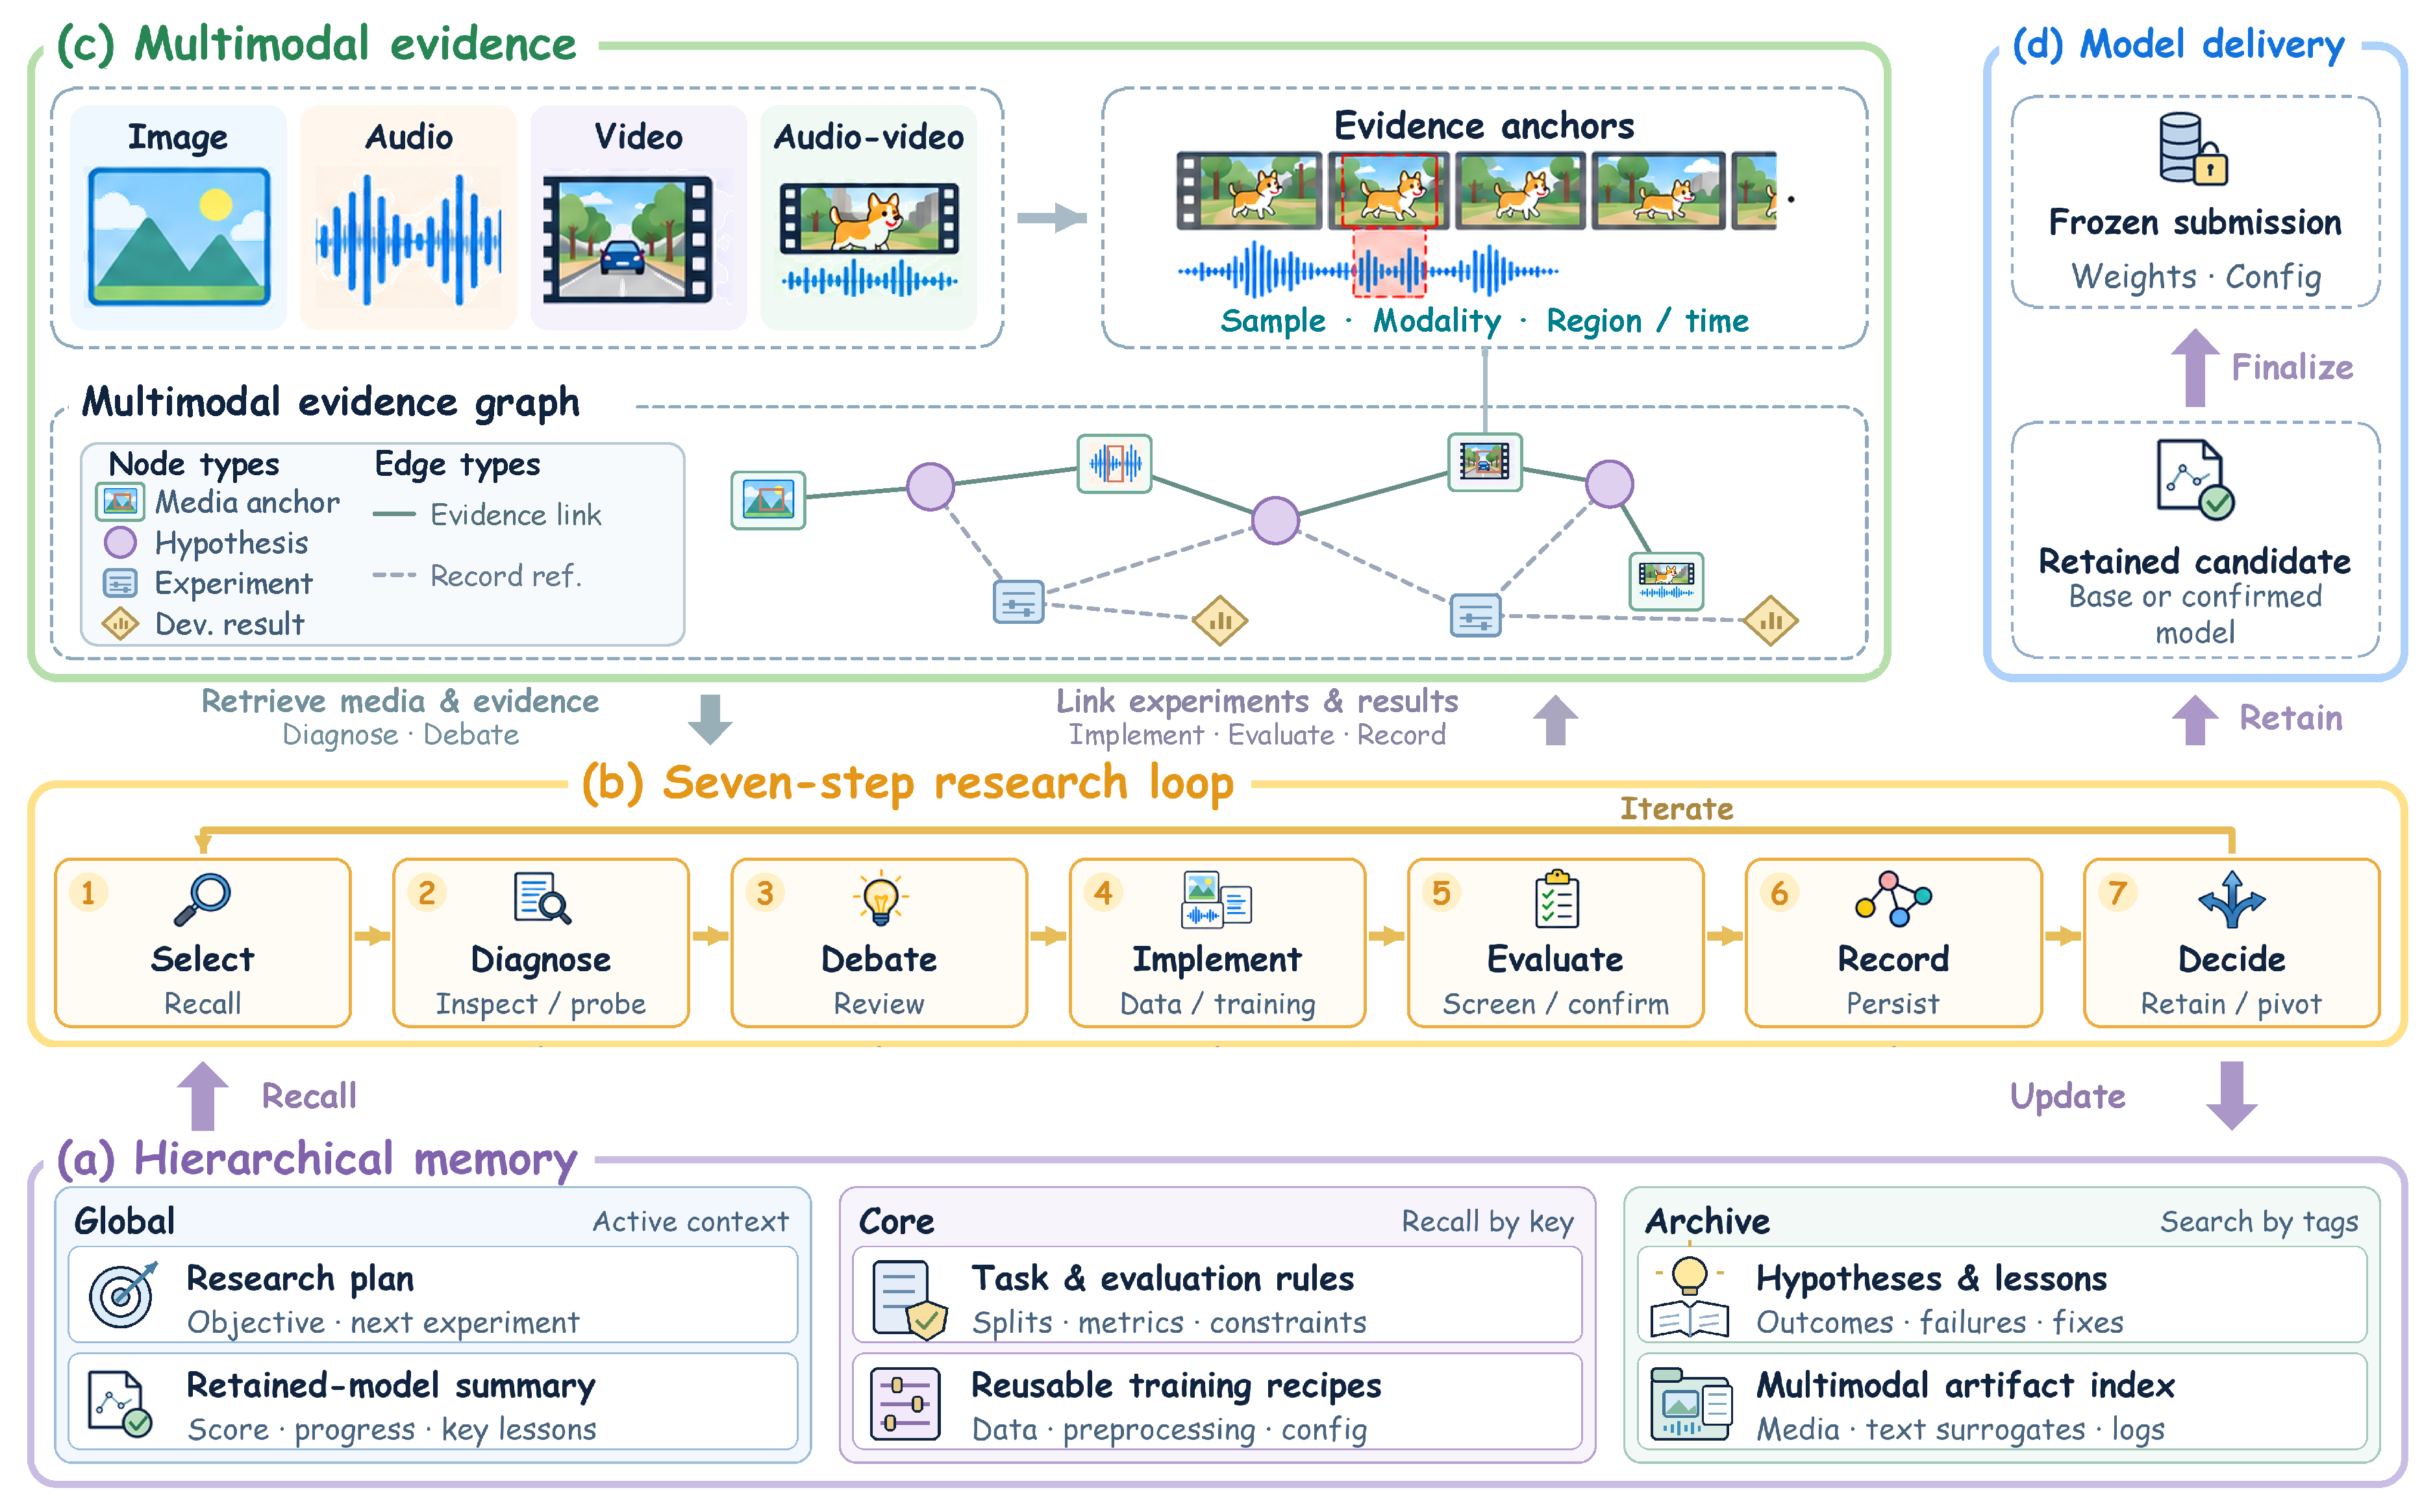
\includegraphics[width=1.0\linewidth]{mile/figures/reference_harness.pdf}
\caption{\textbf{MMResearch framework.} MMResearch coordinates a seven-step research loop (b), using hierarchical memory (a) to guide experimentation and multimodal evidence (c) to connect observations with experimental decisions, then freezes the retained candidate for delivery (d).}
\label{fig:harness}
\end{figure}

\noindent\textbf{Seven-Step Research Loop.}
Each round turns a research direction into an evaluated candidate and a decision (Figure~\ref{fig:harness}b). \textsc{Select} chooses a data- or model-side direction from prior hypotheses and failure records. \textsc{Diagnose} inspects authorized multimodal inputs to investigate the suspected failure. \textsc{Debate} reviews the diagnosis, intervention, feasibility, and risks. \textsc{Implement} executes the intervention and saves a candidate. \textsc{Evaluate} screens and confirms candidates on development data. \textsc{Record} stores configurations, results, and rationales in hierarchical memory. \textsc{Decide} uses confirmation results to promote the candidate, refine the approach, or pivot to another direction; a proxy improvement alone does not justify promotion. A separate checkpoint tracks the retained model, initially the base. Before the budget expires, the controller checks required records and freezes the retained model's weights and configuration for delivery.

\noindent\textbf{Multimodal Evidence.}
The agent inspects authorized image, audio, video, and audio-video inputs through native perception or configured tools. In the \emph{multimodal evidence graph} design (Figure~\ref{fig:harness}c), each \emph{evidence anchor} identifies a source sample, its modality, and a relevant region or time span. When finer localization is unavailable, the anchor refers to the whole image or clip. Direct observations are stored separately from the hypotheses inferred from them. Links connect observations, hypotheses, training interventions, and development-evaluation outcomes, making diagnoses traceable to the underlying media. \textsc{Diagnose} and \textsc{Debate} use the linked observations to review explanations; \textsc{Record} preserves the evidence and outcome links for subsequent rounds. Later rounds can follow these links back to the source media and prior interventions to reassess an earlier diagnosis in light of development results. Held-out test results remain outside this research feedback loop.

\noindent\textbf{Hierarchical Memory.}
\harness{} preserves research context across rounds in three memory tiers (Figure~\ref{fig:harness}a). \emph{Global} maintains the active research plan and a summary of the retained model. \emph{Core} stores task and evaluation rules and reusable training recipes. \emph{Archive} indexes hypotheses, outcomes, failures, and media artifacts. \textsc{Select} retrieves relevant records at the start of a round, and \textsc{Record} updates them with its results and lessons, allowing later experiments to build on earlier findings.

